\documentclass{amsart}

\usepackage[]{mathtools} 
\usepackage[]{cleveref} 
\usepackage[]{color} 
\usepackage[]{tikz} 
\usepackage[]{subcaption} 
\usepackage[backend=biber, style=numeric]{biblatex} 
\bibliography{ivarhs.bib}
\title{Assignment 1 --- MAT-INF4160}
\author{Ivar Haugal{\o}kken Stangeby}
\date{\today}

\begin{document}
\maketitle

\subsection*{Problem 1} 
\label{par:problem_1}

Recall that a \emph{Bernstein polynomial} is a polynomial of the form
\begin{equation}
	\notag
	B_{i}^{n}(x) = {n \choose i} x^i (1 - x)^{n-i}
\end{equation}
where we typically let $x$ live in the unit interval $\left[ 0, 1
\right]$.  We define $n$ to be \emph{degree} of the polynomial, and we
call $B_i^n$ the \emph{$i$'th Bernstein polynomial} of degree $n$ where $i
= 0, \ldots, n$.  Note that by the binomial theorem the $n + 1$ Bernstein
polynomials of degree $n$ sum to $1$ on the unit interval.

By application of the product rule and substitution rule we can
differentiate $B_i^n(x)$ with respect to $x$ which yields
\begin{equation}
	\notag
	\frac{d}{dx}B_i^n(x) = n \left(B_{i-1}^{n-1}(x) - B_{i}^{n-1}(x) \right)
\end{equation}
We seek to show that $B_i^n(x)$ has a unique maximum in the interval $[0, 1]$
with this maximum being $x = i / n$. Note that by the extreme value theorem,
since $B_i^n$ is continuous and $[0, 1]$ is compact, we know that $B_i^n$ does
indeed attain a maximum in $[0, 1]$ but it is not neccessarily unique.

In order to find the maximum, we look at where the derivative is zero.
Consider the derivative of $B_i^n$ where $n \neq 0$. It then suffices to look
at the difference between lower-degree Bernstein polynomials:
\begin{align*}
	{n-1 \choose i-1}x^{i-1}(1 - x)^{n-i} - {n-1 \choose i}x^i(1-x)^{n-i-1} &= 0
\end{align*}
assuming $x \neq 0$ and $x \neq 1$ and we can cancel common terms which yields
\begin{align*}
	\frac{1}{n-1} - x \left( \frac{1}{n - i} + \frac{1}{i} \right) &= 0
\end{align*}
where solving for $x$ gives us $x = i / n$. We have now shown that under the
condition that $x \neq 0$ and $x \neq 1$ the statement holds. Plugging in $x =
0$ and $x = 1$ verifies the claim for those two numbers as well.

\subsection*{Problem 2}\footnote{The solution here is based on the answer
	given to my question posted at \cite{1915642} as well as the
	answer given at \cite{377929}. My initial idea to look at $m+1$'th
	derivatives of $g$ did not lead to anything conclusive.}
	\label{sub:problem_2}

We define the \emph{Bernstein approximation} of a function $f: [0, 1] \to
\mathbb{R}$ of order $n$ as the polynomial
\begin{align*}
	g(x) = \sum^{n}_{i=0} f \left( i / n \right) B_i^n(x).
\end{align*}
We want to show that if $f$ is a polynomial of degree $m \leq n$, then $g$
is also a polynomial of degree $m$. Note first that the \emph{Bernstein
operator} $\mathcal{B}[f]$ sending $f$ to $g$ is \emph{linear}, i.e.,
\begin{equation}
	\notag
	\mathcal{B}\left[x_1f_1 + x_2f_2\right] = x_1\mathcal{B}[f_1] + x_2\mathcal{B}[f_2].
\end{equation}
It therefore suffices to show that the claim holds for $f(x) = x^m$, and
this will simplify the problem a great deal. The overarching strategy here
seems to be to manipulate the expression for $g$ in such a way that we can
consider the coefficients $D_i$ in front of $x^i$ and show that $D_i$ is
in fact zero for $i > m$.

We start by expanding the expression for $g(x)$ with $f$ taken to be $f(x)
= x^m$. This yields
\begin{align*}
	g(x) &= \frac{1}{n^m} \sum^{n}_{i=0} i^m {n \choose i}x^i(1 - x)^{n-i}. \\
	\intertext{Expanding $(1-x)^{n-i}$ using the binomial theorem}
	&= \frac{1}{n^m} \sum^{n}_{i=0} \sum^{n-i}_{j=0} i^m {n \choose i}{n-i \choose j} x^{i + j} (-1)^j
\end{align*}
We can now rewrite the double sum in terms of new summation indices. If we
let $\mathcal{I}$ denote our index set, then $\mathcal{I} = \left\{ (i, j)
\mid i = 0, \ldots n; j = 0, \ldots i \right\}$. This can be rewritten as
$\mathcal{I} = \left\{ (l, k-l) \mid k = 0, \ldots, n; l = 0, \ldots, k
\right\}$. That is, setting $i = l$, $j = k - l$.
\begin{figure}
	\begin{subfigure}[b]{0.4\textwidth}
		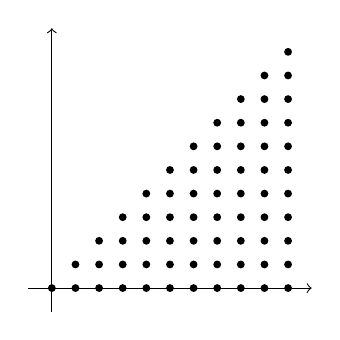
\begin{tikzpicture}[scale=0.3]
			\draw[->] (0, -1) -- (0, 11);
			\draw[->] (-1, 0) -- (11, 0);
			\foreach \i in {0, ..., 10}{
				\foreach \j in {0, ..., \i}{
					\node at (\i, \j) [circle, fill=black, scale=0.3] {};
				}
			}
		\end{tikzpicture}
\end{subfigure}
\begin{subfigure}[b]{0.4\textwidth}
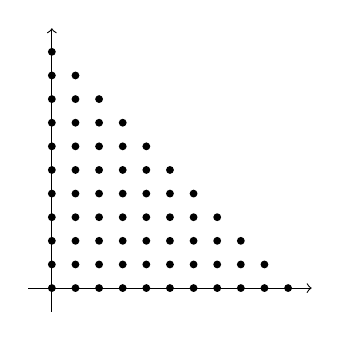
\begin{tikzpicture}[scale=0.3]
\draw[->] (0, -1) -- (0, 11);
\draw[->] (-1, 0) -- (11, 0);
\foreach \i in {0, ..., 10}{
	\foreach \j in {0, ..., \i}{
		\node at (10-\i, \j) [circle, fill=black, scale=0.3] {};
	}
}
\end{tikzpicture}
\end{subfigure}
\caption{Summing over a triangular index set $\mathcal{I}$ in two equivalent
ways.}
\end{figure}
We can with this in mind, rewrite $g(x)$ as
\begin{align*}
	\notag
	g(x) &= \frac{1}{n^m}\sum^{n}_{k=0} \sum^{k}_{l=0} l^m {n \choose k}{k \choose l}(-1)^{k-l}x^k
	\intertext{and separating the independent terms yields} 
	&= \frac{1}{n^m}\sum^{n}_{k=0} {n \choose k}(-1)^kx^k \sum^{k}_{l=0} l^m {k \choose l}(-1)^l.
\end{align*}
It now makes sense to talk about the coefficient of $x^k$, so let $D_k =
\sum^{k}_{l=0}l^m{k \choose l}(-1)^l$. Assume that $k > m$. In order to
show that $D_k = 0$ for $k > m$, define the operator $\mathcal{L}$ by
\begin{equation}
	\notag
	\mathcal{L}[f](x) = x f'(x).
\end{equation}
Furthermore, define the auxilliary functions $p(x) = (x - 1)^k$ and $h(x)
= x^l$. First observe that $\mathcal{L}^m[h](x) = l^mx^l$ and that since
$k > m$, $(x - 1)$ is a factor in $\mathcal{L}^m[p](x)$ so consequently,
$\mathcal{L}^m[p](1) = 0$. Expanding $\mathcal{L}^m[p](1)$ we get
\begin{align*}
	0 &= \mathcal{L}^m[p](1) = \mathcal{L}^m[(x - 1)^k](1) \\
	&= \mathcal{L}^m \left[ \sum^{k}_{i=0} {k \choose i}x^k(-1)^{k-i}\right](1).
	\intertext{Using the fact that $\mathcal{L}$ is linear, we have}
	&= \sum^{k}_{i=0} {k \choose i}(-1)^{k-i} \mathcal{L}^m \left[ x^i \right](1)\\
	&= (-1)^k \sum^{k}_{i=0} {k \choose i}(-1)^ll^m\\
	&= (-1)^k D_k = 0
\end{align*}
so $D_k$ is zero for $k > m$.
\subsection*{Problem 3}
\label{sub:problem_3}

We wish to show that $\Delta^i c_0 = \sum^{i}_{k=0}(-1)^{i-k}{i \choose k}c_k$.
We instead prove a more general claim, namely that
\begin{equation}
	\notag
	\Delta^i c_j = \sum^{i}_{k=0} (-1)^{i-k}{i\choose k}c_{k+j},
\end{equation} and the initial claim will follow with $j = 0$.  We proceed by
induction. The base case consists of showing that the claim holds for $i = 1$.
In this case we have $\Delta c_j = c_{j+1} - c_{j}$ so this holds.  Assume
inductively that the claim holds for the natural number $i$. We then have
\begin{flalign*}
	\notag
	\Delta^{i+1} c_j &= \Delta^{i} c_{j+1} - \Delta^i c_j = \sum^{i}_{k=0} (-1)^{i-k}{i \choose k}\left( c_{k+j+1} - c_{k+j} \right).
	\intertext{Through a change of summation index this is the
	equivalent to}
	&= \sum^{i+1}_{k=1} (-1)^{i-k}{i \choose k-1} c_{k + j} + \sum^{i}_{k=0} (-1)^{i + 1 - k} {i \choose k}c_{k + j}
	\intertext{We now extract the last term from the first sum, and
	the first term from the last sum, which yields}
	&= c_{i + 1 + j} + \left(\sum^{i}_{k=1} \left( {i \choose k - 1} + {i \choose k} \right) (-1)^{i+1-k}c_{k+j}\right) + (-1)^{i+1}c_j.
	\intertext{Using the fact that ${i \choose k - 1} + {i \choose k}
	= {i + 1 \choose k}$ we can write this as}
	&= c_{i + 1 + j} + \left(\sum^{i}_{k=1} {i + 1 \choose k} (-1)^{i+1-k}c_{k+j}\right) + (-1)^{i+1}c_j. \\
	\intertext{Putting it all together, we end up with}
	&=  \sum^{i+1}_{k=0} (-1)^{i + 1 - k} {i + 1 \choose k} c_{k+j},
\end{flalign*}
as we wanted to show. This closes the induction, so if we set $j = 0$, we see
that the initial claim is true: $\Delta^i c_0 =
\sum^{i}_{k=0}(-1)^{i-k}{i \choose k}c_k$.

\subsection*{Problem 4}
\label{sub:problem_4}

We wish to show that
\begin{equation}
	n(n-1) \ldots  (n - k)t^{k+1} = \sum^{n}_{i=0} i(i - 1) \ldots  (i-k)B_i^n(t).
\end{equation}
Note that this always holds for $k \geq n$, so we assume that $k$ is strictly
smaller than $n$.

\printbibliography
\end{document}
